\begin{figure}[t]
\centering
\subfigure[\gls{SLIC}]{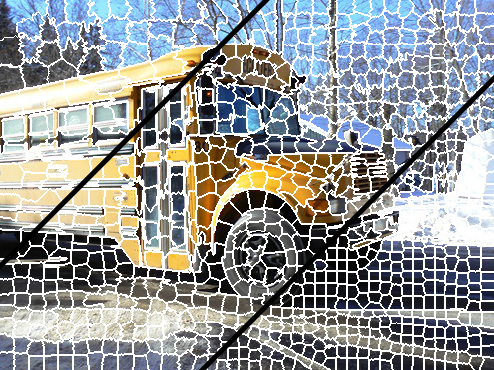
\includegraphics[scale=0.4]{bilder/slic_beispiel}}
\subfigure[Quickshift]{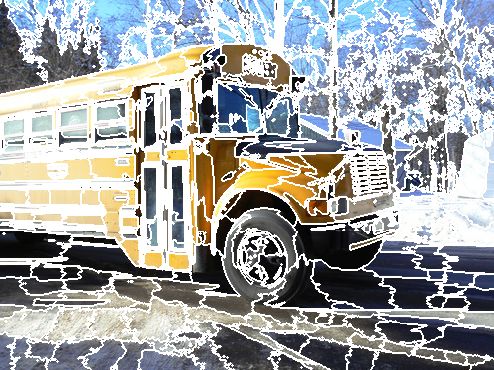
\includegraphics[scale=0.4]{bilder/quickshift_beispiel}}
  \caption[\gls{SLIC} und Quickshift Beispielresultat]{Ein Bus segmentiert über \gls{SLIC} mit jeweils 400, 800 und 1600 Superpixeln (a) sowie über Quickshift mit 600 Superpixeln (b).}
\label{fig:slic_quickshift}
\end{figure}
